%!TEX root = ../main.tex

\chapter{Germanium detector models}%
\label{apdx:gedetav}

As a result of the presence of the \nplus\ contact on the outer surface of the germanium
detectors, the charge-collection efficiency (CCE) differs from unity in the region of the
crystal close to the contact. As a matter of fact, lithium impurities diffused inside the
crystal during the \nplus\ contact fabrication process act as recombination centers for
charge carriers, and thus the CCE curve strongly depends on the lithium concentration
profile. Since part of the charge is lost, events depositing energy in this region are
typically characterized by a lower reconstructed energy, depending on the local CCE. Since
the \pplus\ contact is boron-implanted, it is expected to have a thin dead layer, on the
order of 1~\mum, and it will not be considered in the following. The interested reader is
referred to~\cite{Lehnert2016} for an extensive discussion of the charge-collection
mechanism in germanium detectors and CCE models.

\section{Recommended model from characterization data}%
\label{sec:gedetav:chardata}

\begin{figure}
  \centering
  \includegraphics{setup/gedet-av/tl-model.pdf}
  \caption{%
    Germanium detector active volume model. The charge-collection efficiency is zero by
    definition at the outer surface and remains such through all the `dead layer'. The
    detector is partially active in the `transition layer' region, where the CCE gradually
    increases until reaching its maximal value in the fully active volume.
  }\label{fig:gedetav:tl-model}
\end{figure}

\blocktitle{fully \\ active \\ volume}
The full charge-collection depth (FCCD), defined as the depth at which the CCE reaches
unity, has been estimated for each germanium detector deployed in \gerda\ at the \nplus\
contact during dedicated characterization campaigns. In these measurements, a radioactive
source (e.g.~\Am, \Ba, \Co) is positioned close to the detector surface, and a data sample
is acquired. A comparison between data and Monte Carlo simulations is then performed to
find the FCCD value that best describes data. The recommended FCCD values obtained from
this characterization data are reported in \cref{tab:gedetav:official} and are briefly
described in the following. The \scoax\ values are extracted from \Co\ data as documented
in~\cite{Heider2009}, while the \bege\ values are obtained combining \Am\ and \Ba\
data~\cite{Agostini2019}. \icoax\ values are extracted from \Am\
measurements~\cite{Miloradovic2020}. The \bege\ detectors have been stored at room
temperature in the time interval between their characterization to the deployment in
liquid argon, and must be therefore corrected for the dead-layer growing effect. The
growth speed at room temperature has never been determined rigorously, and the best
available estimate is of about $\sim$$0.1$~mm/yr, with a standard deviation of 0.04~mm/yr
(\cite{Agostini2019} and references therein). The correction is therefore applied
considering the exact time spent by each detector at room temperature together with an
additional systematic uncertainty of 50\%.
\begin{table}
  \centering
  \caption{%
    Recommended full charge-collection depth (FCCD) and dead layer fraction (DLF) values
    for each detector deployed in \gerdatwo, calculated from detector characterization
    data. The \bege\ FCCD values are obtained combining \Am\ and \Ba\
    data~\cite{Agostini2019} while \scoax\ values are extracted from \Co\
    data~\cite{Heider2009}. The \icoax\ values are obtained from \Am\
    data~\cite{Miloradovic2020}. The \bege\ FCCDs are corrected for the dead-layer growing
    effect at room temperature experienced before installment in
    \gerda~\cite{Agostini2019}. The \bege\ uncertainties are split into correlated and
    uncorrelated contributions (FCCD$\protect\substack{+\text{corr}\,+\text{ucorr} \\
    -\text{corr}\,-\text{ucorr}}$). The DLF values have been estimated
    in~\cite{Lehnert2016} and do not include any growing effect at room temperature.
    Detector \GD{02D} does not fully deplete and is therefore excluded from any physics
    analysis~\cite{Agostini2019}.
  }\label{tab:gedetav:official}
  \newcommand{\mes}[3]{\measurement{#1}{#2}{#3}}
\newcommand{\mep}[5]{${#1}\substack{+#2\,+#3 \\ -#4\,-#5}$}

\begin{tabular}{rcc}
  \toprule
  Detector & FCCD (mm)                          & DLF                    \\
  \midrule
  \ANG{1}  & \mep{0.00}{0.00}{0.00}{0.00}{0.00} & --                     \\
  \ANG{2}  & \mep{0.00}{0.00}{0.00}{0.00}{0.00} & --                     \\
  \ANG{3}  & \mep{0.00}{0.00}{0.00}{0.00}{0.00} & --                     \\
  \ANG{4}  & \mep{0.00}{0.00}{0.00}{0.00}{0.00} & --                     \\
  \ANG{5}  & \mep{0.00}{0.00}{0.00}{0.00}{0.00} & --                     \\
  \RG{1}   & \mep{0.00}{0.00}{0.00}{0.00}{0.00} & --                     \\
  \RG{2}   & \mep{0.00}{0.00}{0.00}{0.00}{0.00} & --                     \\
  \midrule
  \GD{00A} & \mep{0.91}{0.15}{0.03}{0.14}{0.05} & \mes{0.17}{0.05}{0.04} \\
  \GD{00B} & \mep{0.00}{0.00}{0.00}{0.00}{0.00} & \mes{0.00}{0.00}{0.00} \\
  \GD{00C} & \mep{0.00}{0.00}{0.00}{0.00}{0.00} & \mes{0.00}{0.00}{0.00} \\
  \GD{00D} & \mep{0.00}{0.00}{0.00}{0.00}{0.00} & \mes{0.00}{0.00}{0.00} \\
  \GD{02A} & \mep{0.00}{0.00}{0.00}{0.00}{0.00} & \mes{0.00}{0.00}{0.00} \\
  \GD{02B} & \mep{0.00}{0.00}{0.00}{0.00}{0.00} & \mes{0.00}{0.00}{0.00} \\
  \GD{02C} & \mep{0.00}{0.00}{0.00}{0.00}{0.00} & \mes{0.00}{0.00}{0.00} \\
  \GD{02D} & \mep{0.00}{0.00}{0.00}{0.00}{0.00} & \mes{0.00}{0.00}{0.00} \\
  \GD{32A} & \mep{0.00}{0.00}{0.00}{0.00}{0.00} & \mes{0.00}{0.00}{0.00} \\
  \GD{32B} & \mep{0.00}{0.00}{0.00}{0.00}{0.00} & \mes{0.00}{0.00}{0.00} \\
  \GD{32C} & \mep{0.00}{0.00}{0.00}{0.00}{0.00} & \mes{0.00}{0.00}{0.00} \\
  \GD{32D} & \mep{0.00}{0.00}{0.00}{0.00}{0.00} & \mes{0.00}{0.00}{0.00} \\
  \GD{35A} & \mep{0.00}{0.00}{0.00}{0.00}{0.00} & \mes{0.00}{0.00}{0.00} \\
  \GD{35B} & \mep{0.00}{0.00}{0.00}{0.00}{0.00} & \mes{0.00}{0.00}{0.00} \\
  \bottomrule
\end{tabular}
\quad
\begin{tabular}{rcc}
  \toprule
  Detector & FCCD (\mum)                        & DLF                    \\
  \midrule
  \GD{35C} & \mep{0.00}{0.00}{0.00}{0.00}{0.00} & \mes{0.00}{0.00}{0.00} \\
  \GD{61A} & \mep{0.00}{0.00}{0.00}{0.00}{0.00} & \mes{0.00}{0.00}{0.00} \\
  \GD{61B} & \mep{0.00}{0.00}{0.00}{0.00}{0.00} & \mes{0.00}{0.00}{0.00} \\
  \GD{61C} & \mep{0.00}{0.00}{0.00}{0.00}{0.00} & \mes{0.00}{0.00}{0.00} \\
  \GD{76B} & \mep{0.00}{0.00}{0.00}{0.00}{0.00} & \mes{0.00}{0.00}{0.00} \\
  \GD{76C} & \mep{0.00}{0.00}{0.00}{0.00}{0.00} & \mes{0.00}{0.00}{0.00} \\
  \GD{79B} & \mep{0.00}{0.00}{0.00}{0.00}{0.00} & \mes{0.00}{0.00}{0.00} \\
  \GD{79C} & \mep{0.00}{0.00}{0.00}{0.00}{0.00} & \mes{0.00}{0.00}{0.00} \\
  \GD{89A} & \mep{0.00}{0.00}{0.00}{0.00}{0.00} & \mes{0.00}{0.00}{0.00} \\
  \GD{89B} & \mep{0.00}{0.00}{0.00}{0.00}{0.00} & \mes{0.00}{0.00}{0.00} \\
  \GD{89C} & \mep{0.00}{0.00}{0.00}{0.00}{0.00} & \mes{0.00}{0.00}{0.00} \\
  \GD{89D} & \mep{0.00}{0.00}{0.00}{0.00}{0.00} & \mes{0.00}{0.00}{0.00} \\
  \GD{91A} & \mep{0.00}{0.00}{0.00}{0.00}{0.00} & \mes{0.00}{0.00}{0.00} \\
  \GD{91B} & \mep{0.00}{0.00}{0.00}{0.00}{0.00} & \mes{0.00}{0.00}{0.00} \\
  \GD{91C} & \mep{0.00}{0.00}{0.00}{0.00}{0.00} & \mes{0.00}{0.00}{0.00} \\
  \GD{91D} & \mep{0.99}{0.16}{0.03}{0.16}{0.06} & \mes{0.36}{0.04}{0.03} \\
  \midrule
  \IC{48A} & \mep{0.00}{0.00}{0.00}{0.00}{0.00} & --                     \\
  \IC{48B} & \mep{0.00}{0.00}{0.00}{0.00}{0.00} & --                     \\
  \IC{50A} & \mep{0.00}{0.00}{0.00}{0.00}{0.00} & --                     \\
  \IC{50B} & \mep{0.00}{0.00}{0.00}{0.00}{0.00} & --                     \\
  \IC{74A} & \mep{0.00}{0.00}{0.00}{0.00}{0.00} & --                     \\
  \bottomrule
\end{tabular}

\end{table}

\blocktitle{transition \\ layer}
The region enclosed by the detector surface and the FCCD is, of course, not completely
dead, and regions with reduced CCE are expected. The CCE curve in this region strongly
depends on the lithium concentration profile, which is in turn strongly dependent on the
diode fabrication process (initial lithium concentration at the surface, thermal annealing
cycles etc.) and is \emph{a priori} different for each detector. As a consequence, the
transition region must be characterized for each detector individually, i.e.~in a similar
way as FCCD is determined from external source data.
\newpar
It is important to stress here that a precise characterization of the transition layer is
not needed for the \onbb\ analysis, as the introduction of a partially-active region above
the FCCD results in hypothetical, new \onbb\ events below the \qbb. \onbb\ events
originating in this transition region would in fact be detected with an effectively lower
energy and therefore `get out' of the gaussian peak at \qbb, which is what the experiment
looks for. In other words, the presence of a non-null transition layer would have no
impact on the signal detection efficiency defined for the \onbb\ analysis. Constraining
the CCE curve is instead important for the \nnbb\ analysis. Different transition layer
models result in shape distortions of the \nnbb\ energy distribution that can potentially
mimic the presence of new-physics phenomena (e.g.~those considered in
\cref{sec:nbb:0nbbx,sec:nbb:2nbbLV})\footnote{%
  Technically, the size of the transition region marginally affects also the \thalftwo\
  estimate, since it depends on the total number of detected \nnbb\ events, which
  increases with the size of the transition region. This effect, however, is negligible
  compared to the uncertainty induced by the FCCD estimates.
}. The potential systematic effect due to the uncertainties in the CCE curve determination
is investigated in \cref{sec:2nbb-ana:systematics}.
\newpar
An attempt to determine the CCE curve for \gerda's \bege\ detectors has been carried on
in~\cite{Lehnert2016}. A simple linear model (the one shown in
\cref{fig:gedetav:tl-model}) has been considered at first. Once the FCCD is fixed, as it
is clear from the formulation of the model, the only parameter that needs to be
constrained is the starting point of the transition region, i.e.~the dead layer thickness
(DLT). Monte Carlo simulations performed with different DLTs have been compared to \Am\
data in order to determine the dead-layer fraction (DLF), defined as
\[
  \text{DLF} = \frac{\text{DLT}}{\text{FCCD}} \in [0,1] \;,
\]
For each \bege\ detector. The results are reproduced in \cref{tab:gedetav:official}. Since
the effect of the lithium concentration profile evolution at room temperature on the
transition region is not known, these values have not been corrected. A more complex
transition layer model has been also derived from first principles in~\cite{Lehnert2016},
but it requires special PSD data from other radioactive sources (i.e.~\aoe\ from
\nuc{Sr}{90} in~\cite{Lehnert2016}) that is available just for \GD{91C}.

\blocktitle{known \\ issues}
Unfortunately, the active volume model presented above suffers from many uncertainties and
cannot be fully trusted. A systematic discrepancy between FCCD values obtained from
different radioactive sources (\Am, \Ba\ and \Co) has been highlighted and
discussed~\cite{Lehnert2016}, but no convincing explanation of its origin has been
formulated yet. Moreover, the fact that \bege\ detectors were stored at room temperature
for a significant amount of time after being carefully characterized poses an additional
question mark on these FCCD values, as the growing effect has never been carefully studied
in detail. In particular, the size of the transition region extracted from the
characterization data must also be affected by the evolution of the lithium concentration
profile in some way, and cannot be left uncorrected when considering data collected in the
\gerda\ cryostat. Finally, the linear transition layer model could be a bad approximation
in some detectors. An evidence for the presence of these systematic biases lies in the
results of the background model presented in \cref{chap:bkg:raw:ph2}, which yields
incompatible \thalftwo\ estimates from different detector types. More evidence in support
of this discrepancy and possible solutions will be presented in the following sections.

\section{Tuning the \bege\ model on calibration data}%
\label{sec:gedetav:calib-optim}

The effect of the transition region size on the event energy spectrum is particularly
strong in the lower tail of intense \g\ peaks. Full-energy events interacting in the
transition region are reconstructed with a smaller effective energy, and are therefore
shifted out of the peak. The high-statistics \Tl\ 2615~keV line from calibration data is
an interesting sample that can be used to determine the size of the transition region.
Data from the special \Th\ calibration run 68\footnote{%
  As documented in \cref{sec:bkg:lar:ph2:pcalib}, data from run 68 has been collected with
  low-activity $\mathcal{O}(1)$~kBq \Th\ sources, to study the performance of the liquid
  argon veto system. Since in these experimental conditions the rate of pile-up events is
  much lower than in regular calibrations, this data set is more suited to a comparison
  with Monte Carlo simulations.
} collected by the \GD{02A} detector is shown in the left-hand side of
\cref{fig:gedetav:calib-optim-example}, in red. Pdfs corresponding to different sizes of
the transition region (DLF) are overlaid to demonstrate the effect on the low side of the
full-energy peak.
\begin{figure}
  \centering
  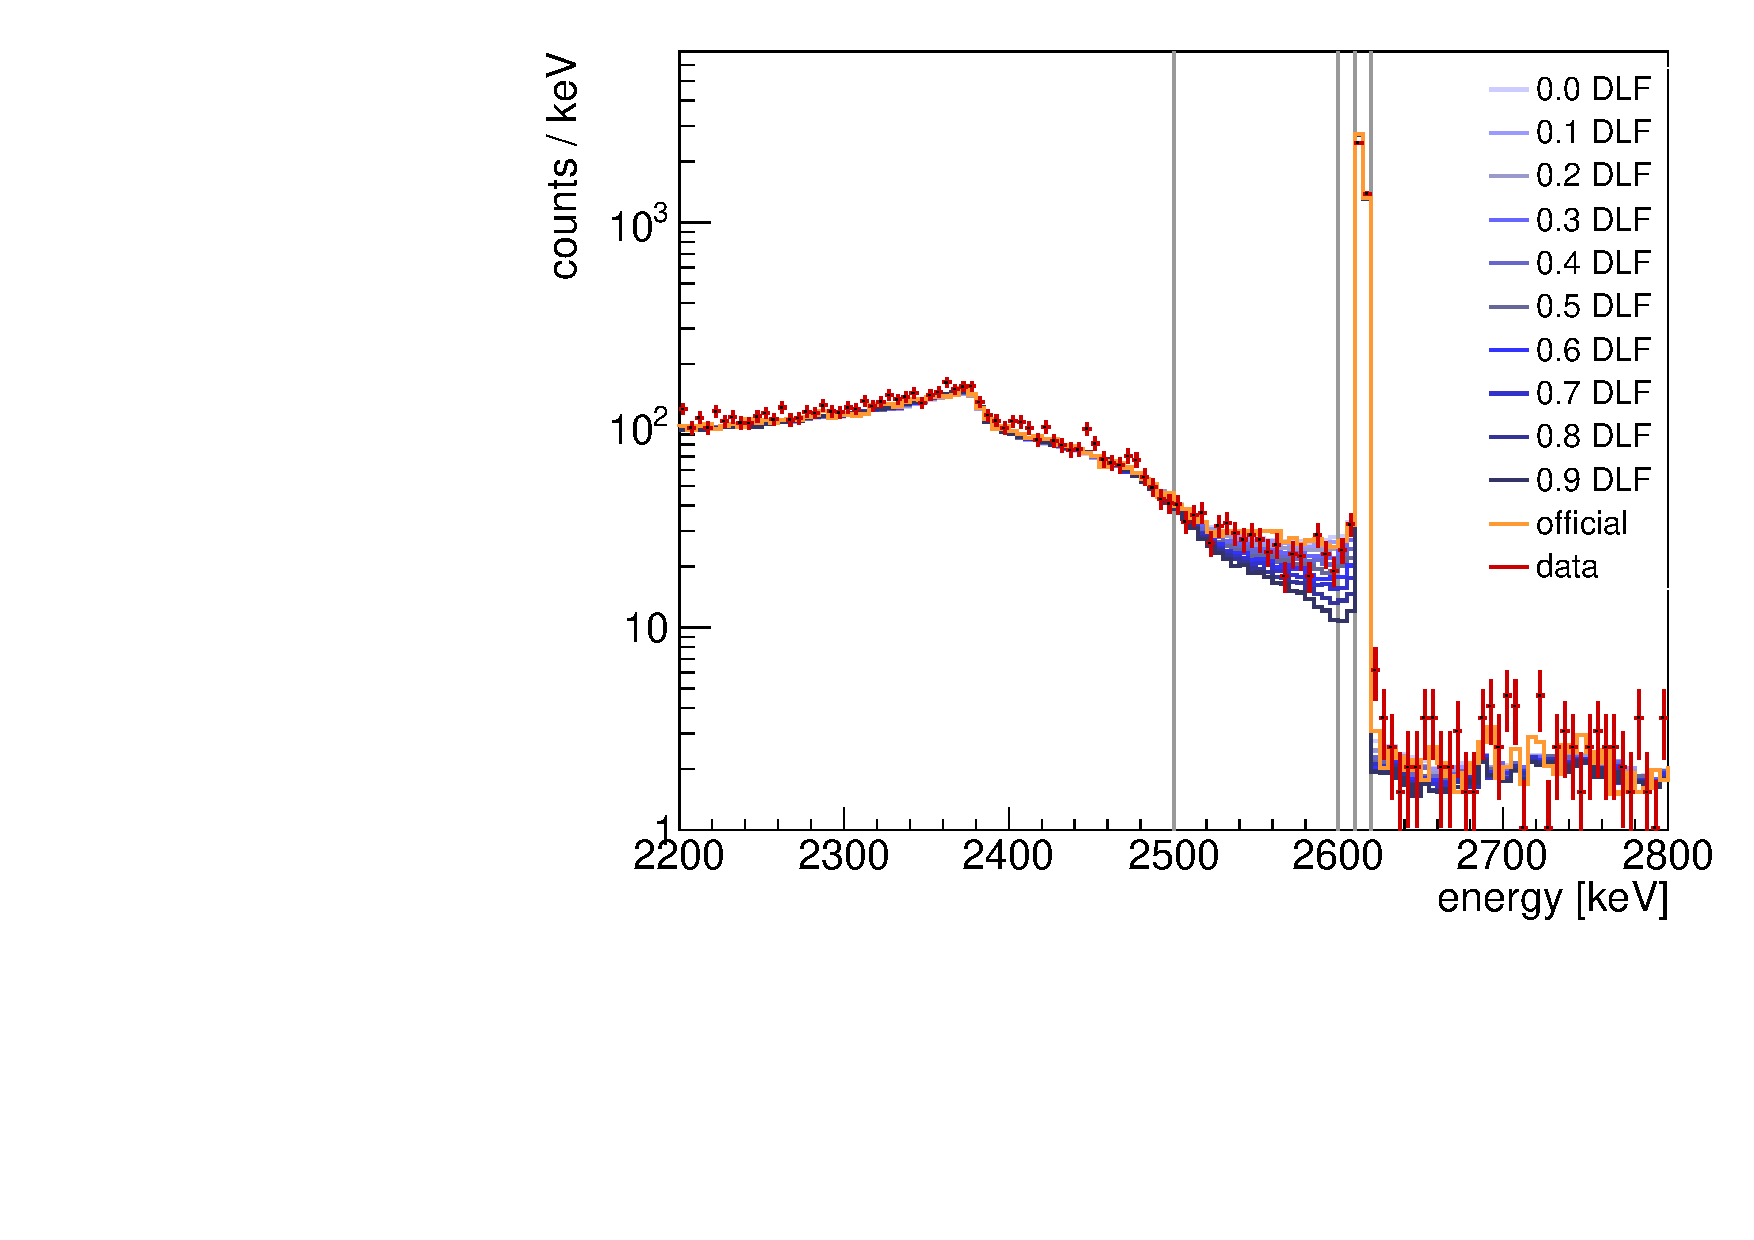
\includegraphics[width=0.46\textwidth]{plots/gedet-av/GD02A-tl-peak.pdf}%
  \hspace{0.07\textwidth}%
  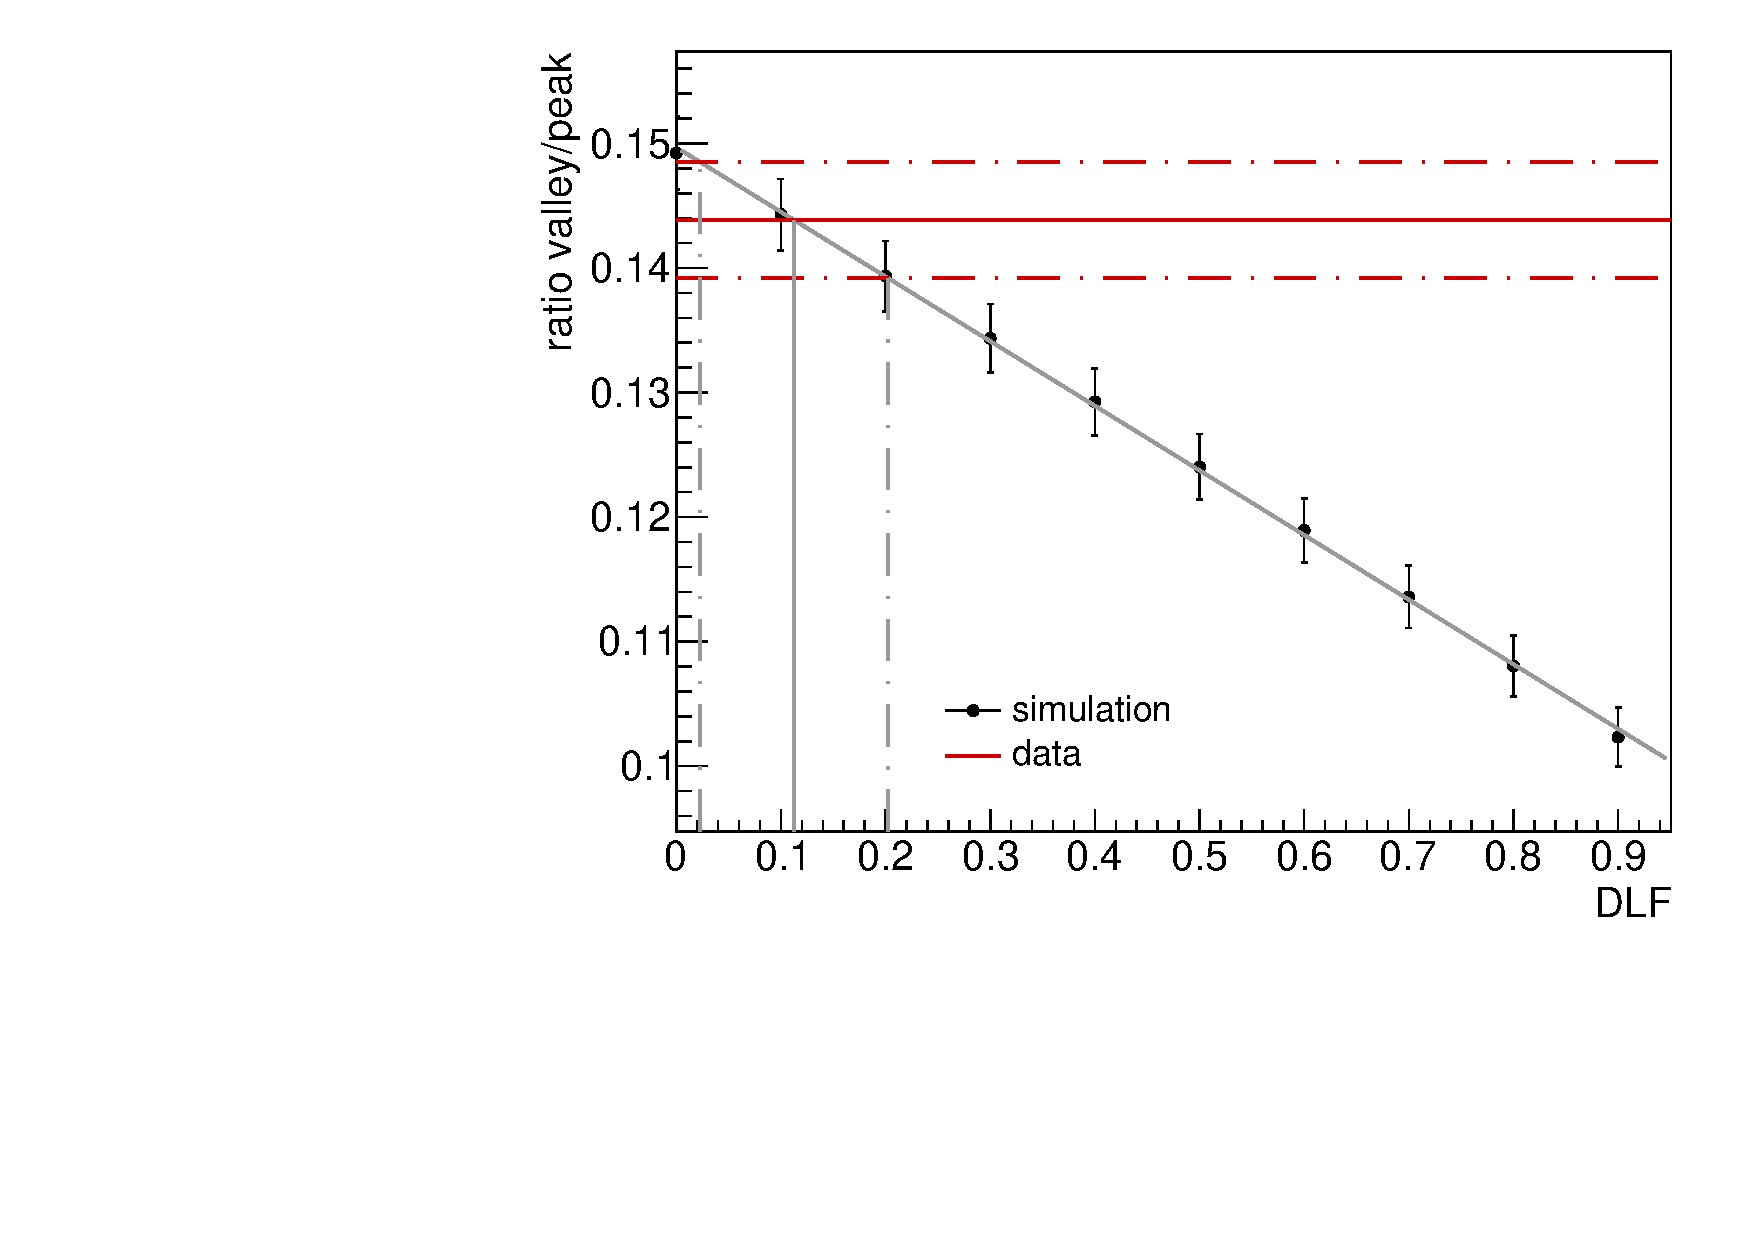
\includegraphics[width=0.46\textwidth]{plots/gedet-av/GD02A-optimization.pdf}
  \caption{%
    Example optimization of the dead-layer fraction for detector \GD{02A}. Left: close-up
    of the energy spectrum in the \Tl\ FEP region. The data (red) is compared against
    simulations with different DLF values, from 0 to 0.9 in steps of 0.1. The pdf
    corresponding to the recommended DLF value (\cref{tab:gedetav:official}) is
    highlighted in orange. The energy regions used to compute the $V/P$ observable are
    shown in grey. Right: extraction of the optimal DLF value by interpolating the
    simulation results. The statistical uncertainties are plot in dashed lines.
  }\label{fig:gedetav:calib-optim-example}
\end{figure}
\newpar
To determine the optimum transition region size the observable $V/P$ is defined, where $V$
(valley) and $P$ (peak) are the total number of counts in the $[2500, 2600]$~keV and
$[2610, 2620]$~keV regions, respectively (the two energy ranges are highlighted in grey in
\cref{fig:gedetav:calib-optim-example}, left). The uncertainty on $V/P$ is obtained by
error propagation of the Poisson uncertainties on $V$ and $P$. Pdfs with dead-layer
fractions from 0 to 0.9 in steps of 0.1 and the FCCDs fixed to the official values in
\cref{tab:gedetav:official} have been produced for each detector, in order to obtain the
predicted $V/P$ values. Since $V/P$ is observed to change linearly upon the dead-layer
fraction, a linear interpolation is performed between the simulated values. The result is
depicted in \cref{fig:gedetav:calib-optim-example}, on the right, for detector \GD{02A}.
Finally, the value of the observable is calculated from data (grey lines) and compared
against the interpolation result in order to find the optimum dead-layer fraction value
(red lines). The results are reported in \cref{tab:gedetav:calib-optim} for each
detector and in \cref{fig:gedetav:calib-optim}, where they are compared with the
dead-layer fractions extracted from detector characterization data. The latter look
clearly underestimated, possibly because of the effect of the \nplus\ contact growth at
room temperature, which has never been studied in the transition region.
\begin{table}
  \centering
  \caption{%
    \bege\ dead-layer fractions obtained from special \Th\ calibration data (run 68).
    Detector \GD{02D} does not fully deplete~\cite{Agostini2019} and is excluded from the
    analysis. Detectors marked with an asterisk ($^*$) are switched off or unusable in run
    68.
  }\label{tab:gedetav:calib-optim}
  \newcommand{\mes}[3]{\measurement{#1}{#2}{#3}}

\begin{tabular}{rc}
  \toprule
  Detector & DLF                    \\
  \midrule
  \GD{00A} & \mes{0.17}{0.05}{0.04} \\
  \GD{00B} & \mes{0.00}{0.00}{0.00} \\
  \GD{00C} & \mes{0.00}{0.00}{0.00} \\
  \GD{00D} & \mes{0.00}{0.00}{0.00} \\
  \GD{02A} & \mes{0.00}{0.00}{0.00} \\
  \GD{02B} & \mes{0.00}{0.00}{0.00} \\
  \GD{02C} & \mes{0.00}{0.00}{0.00} \\
  \GD{02D} & \mes{0.00}{0.00}{0.00} \\
  \GD{32A} & \mes{0.00}{0.00}{0.00} \\
  \GD{32B} & \mes{0.00}{0.00}{0.00} \\
  \bottomrule
\end{tabular}
\quad
\begin{tabular}{rcc}
  \toprule
  Detector & DLF                    \\
  \midrule
  \GD{32C} & \mes{0.00}{0.00}{0.00} \\
  \GD{32D} & \mes{0.00}{0.00}{0.00} \\
  \GD{35A} & \mes{0.00}{0.00}{0.00} \\
  \GD{35B} & \mes{0.00}{0.00}{0.00} \\
  \GD{35C} & \mes{0.00}{0.00}{0.00} \\
  \GD{61A} & \mes{0.00}{0.00}{0.00} \\
  \GD{61B} & \mes{0.00}{0.00}{0.00} \\
  \GD{61C} & \mes{0.00}{0.00}{0.00} \\
  \GD{76B} & \mes{0.00}{0.00}{0.00} \\
  \GD{76C} & \mes{0.00}{0.00}{0.00} \\
  \bottomrule
\end{tabular}
\quad
\begin{tabular}{rcc}
  \toprule
  Detector & DLF                    \\
  \midrule
  \GD{79B} & \mes{0.00}{0.00}{0.00} \\
  \GD{79C} & \mes{0.00}{0.00}{0.00} \\
  \GD{89A} & \mes{0.00}{0.00}{0.00} \\
  \GD{89B} & \mes{0.00}{0.00}{0.00} \\
  \GD{89C} & \mes{0.00}{0.00}{0.00} \\
  \GD{89D} & \mes{0.00}{0.00}{0.00} \\
  \GD{91A} & \mes{0.00}{0.00}{0.00} \\
  \GD{91B} & \mes{0.00}{0.00}{0.00} \\
  \GD{91C} & \mes{0.00}{0.00}{0.00} \\
  \GD{91D} & \mes{0.00}{0.00}{0.00} \\
  \bottomrule
\end{tabular}

\end{table}
\begin{figure}
  \centering
  \includegraphics{plots/gedet-av/calib-optim-results.pdf}
  \caption{%
    Comparison between the recommended DLF values (extracted from detector
    characterization data) and the ones extracted by analyzing the low energy tail of the
    \Tl\ full-energy peak in calibration data. Some values are missing because of
    detectors for which no data is available.
  }\label{fig:gedetav:calib-optim}
\end{figure}
\newpar
Unfortunately, not all detectors were active during run 68. Some of them were switched off
because of hardware instabilities and some of them were not usable because of unstable
energy calibration. Since no data is available for these detectors, an educated guess is
made by assuming a dead-layer fraction equal to an average value. This average value is
calculated by repeating the $V/P$ analysis on the \bege\ summed energy spectrum, and by
varying the simulated dead-layer fraction consistently in all detectors (i.e.~all \bege\
dead-layer fractions set to 0.0, 0.1, \ldots, 0.9). The obtained effective dead-layer
fraction is
\[
  0.529 \pm 0.016 \;,
\]
which carries a smaller uncertainty because of the higher statistics in the data
sample\footnote{%
  This effective dead-layer fraction value is used as an educated guess for detectors in
  the \nnbb\ analysis (\cref{chap:2nbb-ana}) that were inactive in run 68. This assumption
  holds well if only the combined \bege\ energy spectrum is considered in the analysis.
  Moreover, the obtained effective uncertainty is adopted in the estimation of the systematic
  uncertainty contribution from the transition layer model, as it represents the average
  potential distortion seen in the combined energy spectrum.
}.

\section{Insights from \Arl\ data}%
\label{sec:gedetav:ar39}

The \gerda\ event spectrum is dominated, at low energies, by \Arl-decay events. This
unstable nucleus is naturally present in the atmosphere and is cosmogenically activated.
It decays to the ground state of $^{39}$K via $\upbeta^-$ decay with a half-life of
269(3)~yr and Q-value of 656(5)~keV~\cite{Wang2017}. Being commercial liquid argon distilled from air, it
naturally contains a fraction of \Arl, whose activity has been estimated to be of about
1~Bq/kg by various experiments~\cite{Ajaj2019, Calvo2017, Benetti2006, Loosli1983}. The
\Arl\ energy spectrum of events collected by \gerda\ in the first part of \phasetwo\ has
been partly published in~\cite{Agostini2020}.
\newpar
The \b\ particle emitted in the \Arl\ decay can be detected directly or indirectly in
\gerda. In the first case the electron has to directly reach the detector active volume.
Since a \b\ particle of that energy has a mean range in germanium of less than 100~\mum\
and the \nplus\ contact is typically several hundreds of \mum\ thick, the only way is
through the \pplus\ electrode. For the same reason, the mother \Arl\ nucleus must decay
very close to the detector surface, i.e.~less than 1~mm far from it. Being the \pplus\
contact a small fraction of the total detector surface, the \b\ component of the \Arl\
spectrum is expected to be sub-dominant or even negligible for point-like contact
detectors such as \bege{}s or \icoax{}s (c.f.r~\cref{fig:gedetav:ar39:distortions}, left).
\newpar
\Arl\ electrons typically emit \emph{bremsstrahlung} radiation in LAr that can reach the
detector active volume: this is referred as the `indirect' detection method. Since the
photon absorption length in germanium and liquid argon is much longer than the electron
absorption length, \Arl\ decays originating much further from the detector surface can be
detected. Moreover, \emph{bremsstrahlung} photons can interact with the whole detector
volume, and thus constitute a `volume probe'. It follows from what stated above that the
\g\ component largely dominates the \Arl\ event spectrum
(c.f.r.~\cref{fig:gedetav:ar39:distortions}, left).

\begin{figure}
  \centering
  \includegraphics{plots/gedet-av/ar39-spectrum.pdf}%
  \includegraphics{plots/gedet-av/ar39-distortions.pdf}
  \caption{%
    Left: decomposition of the \Arl\ energy spectrum as seen by all \gerda\ detectors into
    \b\ and \g\ components. Center and right: Impact of different linear transition layer
    model (\cref{fig:gedetav:tl-model}) parameters on the \Arl\ energy spectrum shape,
    keeping the \Arl\ activity in LAr fixed. Left: the dead layer fraction (DLF) is fixed
    to 1 (i.e.~hard step model) and the full charge-collection depth (FCCD) is varied
    between 0.3~mm and 1.5~mm in steps of 0.1~mm. Right: the FCCD is fixed to 0.9~mm and
    the DLF is varied between 0 (i.e.~no dead layer) and 1 (i.e.~no transition layer).
  }\label{fig:gedetav:ar39:distortions}
\end{figure}

\blocktitle{active \\ volume \\ model}
The \Arl\ spectral shape is strongly affected by the germanium detector's active volume
model, as it will be demonstrated in the following. This high-statistics data sample
collected by \gerda\ offers the interesting possibility to tune the active volume model on
a detector-by-detector basis. Let's consider, for the sake of simplicity, the simple linear
transition layer model depicted in \cref{fig:gedetav:tl-model} for the \nplus\ contact.
The effects of variations of its two parameters (the FCCD and the DLF) are shown in
\cref{fig:gedetav:ar39:distortions}. Varying the FCCD (and keeping the DLF fixed at 1,
i.e.~no transition layer) has of course the effect of changing the number of detected
\Arl\ events, but introduces a shape distortion too. The effect of the DLF seems to be
more localized in the low side of the distribution. Clearly, the more the transition layer
extends closer to the surface, the more events with incomplete charge collection appear at
lower energies. Remarkably, both parameters seems to shift the position of the maximum of
the distribution.

\blocktitle{tuning the \\ model}
An attempt to fit the \Arl\ energy spectrum and extract FCCD and DLF values for each
detector has been carried on, whose preliminary results are presented here. The
\phasetwop\ data set (\gexpophasetwopbkg) has been considered, as the germanium detectors
energy threshold has been kept low enough (about 40~keV) for the whole data taking. No LAr
veto cut or PSD cut has been applied, as the corresponding Monte Carlo model is not known
in sufficient detail yet or is completely missing. Each detector collected more than $5
\cdot 10^4$ events below 200~keV, where the bulk of the \Arl\ events is located.
\newpar
A set of \Arl\ pdfs has been generated for each detector separately and considering
different combinations of FCCD and DLF values. In this preliminary setting, FCCDs and DLFs
have been sampled in discrete steps of 0.1~mm and 0.1, respectively. Together with the
signal pdf (\Arl), the most prominent background pdfs in the considered energy region have
been generated.  Specifically, \Pbh\ and \Bih\ in the detector cabling, \nnbb\ in
germanium, \kvz\ in liquid argon and \kvn\ in the mini-shrouds. \Arh, which decays into
\kvz\ by emitting a \b\ particle with a Q-value of 599(6)~keV~\cite{Wang2017} which is
very close to the \Arl\ Q-value, has not been considered as its activity in LAr is
negligible, compared to \Arl\ (less than 43~\mubq/kg~\cite{Ashitkov2003}). The \Kr\
contribution has also been discarded because it is highly localized at 514~keV, in
correspondence with its only \g\ line, and does not contribute significantly to the rest
of the energy spectrum\footnote{%
  \Kr\ disintegrates by \b\ emission mainly to the ground state of \nuc{Rb}{85}. Its
  activity in the atmosphere is of the order of 1 Bq/m$^3$, with a half-life of nearly
  11~yr. Its energy spectrum is characterized by a strong \g\ line at 514~keV, compared to
  the Compton and \b\ components. The distillation procedure for the production of liquid
  argon substantially reduces the \Kr\ fraction, and the residual \Kr\ in liquid argon may
  vary in different batches of liquid~\cite{Benetti2006}. A rough estimate of its
  activity in the liquid argon in the \gerda\ cryostat obtained by comparing the simulated
  \Kr\ pdf to the 514~keV line count rate yields 2.3(3)~mBq/kg.
}. To find the
combination of FCCD and DLF that best describes the data, first the background of
the \Arl\ event distribution is fixed at the results of the background model
presented in \cref{chap:bkg:raw:ph2}. Then, for each detector separately, the \Arl\
activity, the FCCD and DLF values are adjusted in order to reproduce the shape of the
energy spectrum and the total number of counts. Since activities in the 1.3--1.4~Bq/kg range
seem to reasonably describe data from all detectors, the same value of 1.35~Bq/kg is
preliminary set for all of them. The results of this manual optimization are shown in
\cref{fig:gedetav:spectra-optim-1,fig:gedetav:spectra-optim-2,fig:gedetav:spectra-optim-3,fig:gedetav:spectra-optim-4},
including the 68\%, 95\% and 99\% confidence intervals that highlight the magnitude of
statistical fluctuations in data. The obtained FCCD and DLF values are compared to the
official values from detector characterization data (where available) in
\cref{fig:gedetav:ar39-results}. It is stressed here that these results are preliminary
and qualitative, as they have not been extracted by means of a careful analysis, which
includes the evaluation of the systematic uncertainties. Note that data is not available
for some detectors that have not been deployed in \phasetwop\ (\ANG{1}) or were switched
off because of hardware instabilities (\ANG{5} and \IC{48B}).

\blocktitle{results}
Starting from the FCCD values, it is interesting to note the high compatibility between
the characterization data and the \Arl\ data for \icoax\ detectors. Indeed, these are the
most precisely-characterized and newly-produced detectors deployed in \gerda. In contrast,
the \Arl\ data analysis reports quite different FCCDs for some \scoax\ detectors, but the
uncertainty on their official estimate is large enough to account for such a deviation.
The situation changes again for \bege\ detectors, in which the new values are almost
always higher than the official estimates and incompatible with them. This discrepancy
could be motivated by the observation that these detectors have been stored at room
temperature, after being characterized, for 2--3 years, a time in which the lithium
concentration profile in the \nplus\ contact could have grown at a different rate than
what has been suggested in the past (\cite{Agostini2019} and references therein). For what
concerns the \bege\ dead-layer fraction values, the \Arl\ analysis results are
systematically higher than the old estimates. This finding is in agreement with what
already seen in calibration data (\cref{sec:gedetav:calib-optim}), and could again be
motivated by the fact that the dead-layer growth model has never been studied in detail
with experimental data.
\newpar
As already mentioned, an \Arl\ activity in the 1.3--1.4~Bq/kg range is needed to reproduce
the observed count rate, given the transition layer model that best reproduces the energy
spectrum shape. This result is in contrast with what reported by other experimental
efforts~\cite{Ajaj2019, Calvo2017, Benetti2006, Loosli1983}, which quote an activity of
about 1~Bq/kg. Considering that an independent analysis of \gerda\ \phaseone\ data
(private communications) seems to obtain the same result and there is no reason to
hypothesize that the argon deployed in \gerda\ has a naturally-higher \Arl\ activity, the
explanation might lie in the different experimental conditions in which \gerda\ operates,
compared to other experiments. However, no convincing hypothesis have been formulated nor
tested yet.

\begin{figure}
  \centering
  \includegraphics{plots/gedet-av/ar39-results.pdf}
  \caption{%
    Comparison between the recommended FCCD and DLF values (extracted from detector
    characterization data and used for the \onbb\ analysis) and the ones extracted by
    analyzing the shape of the \Arl\ energy spectrum. The width of the red bars does not
    represent an uncertainty (see text). Note that DLFs have not been estimated for
    \scoax{}s and \icoax{}s and that some FCCD values from \Arl\ are missing because of
    detectors for which no data is available.
  }\label{fig:gedetav:ar39-results}
\end{figure}

\blocktitle{systematic \\ uncertainties}
There are systematic effects that might play a significant role in this analysis and that
could not be studied with the attention they deserve. These results are indeed preliminary
and should be taken with a grain of salt. Nevertheless, a tentative list of the main
sources of systematic biases is given here for completeness.
\begin{description}
  \item[Quality cuts] The effectiveness of the quality cuts has never been verified in the
    \Arl\ energy region, where a large fraction of the total number of unphysical events
    can be expected. A degrading quality cuts efficiency around the energy threshold might
    induce deformations of the event energy distribution.
  \item[Energy scale and resolution] The correctness of the calibration and resolution
    curves of the germanium detector has never been investigated in detail at such low
    energies. The lowest \g\ line included in the calibration analysis is in fact at
    583~keV, which is even higher than the \Arl\ Q-value. As it can be speculated from
    \cref{fig:gedetav:ar39:distortions}, a systematic shift in the energy scale or
    resolution below the \Arl\ Q-value could mimic distortions corresponding to FCCD
    shifts.
  \item[Transition layer model] A linear model for the CCE in the transition region has
    been used to keep the analysis simple. However, as it can be easily noticed by
    observing data close to the energy threshold, the approximation does not hold
    perfectly throughout the whole \Arl\ energy spectrum. More realistic models should be
    studied in order to asses whether the linear model introduces a severe bias in the
    results.
  \item[Background model] systematic effects arising from an incomplete or inexact
    background model in the low energy region cannot be excluded. As instance, a \Kr\
    contribution is known to be present in LAr (\g\ line at 514~keV) but is ignored in the
    present analysis. A fit of the \Kr\ pdf to the \g\ line visible in data, however,
    suggests a negligible contribution.
  \item[\Arl\ spectrum theoretical shape] The dynamics of the first-forbidden unique
    $\upbeta^-$ decay of \Arl\ are not known in great detail, from a theoretical point of
    view~\cite{Kostensalo2017}. The impact of different numerical calculations should be
    considered when performing such a shape analysis on its energy spectrum. However,
    judging from the order of magnitude of the distortions shown in~\cite{Kostensalo2017},
    this theoretical uncertainty should have a negligible impact.
\end{description}

These qualitative results, despite not being obtained within a robust statistical
framework and despite the lack of a careful study of potential sources of systematic
uncertainties, show all the potential of an \Arl\ data analysis. This decaying nucleus
offers the unique possibility to characterize the active volume of germanium detectors
\emph{in situ} and in a clear way, without recurring to dedicated characterization
campaigns prior installment in the experimental apparatus.

\begin{figure}
  \centering
  \includegraphics{plots/gedet-av/ar39-spectra-optim-1.pdf}
  \caption{%
    \gerda\ \phasetwop\ data (\gexpophasetwopbkg) in the $[40, 250]$~keV energy range and
    best-matching Monte Carlo model determined by adjusting the transition layer model.
    The corresponding FCCD and DLF values are shown in \cref{fig:gedetav:ar39-results}.
  }\label{fig:gedetav:spectra-optim-1}
\end{figure}

\begin{figure}
  \centering
  \includegraphics{plots/gedet-av/ar39-spectra-optim-2.pdf}
  \caption{%
    \gerda\ \phasetwop\ data (\gexpophasetwopbkg) in the $[40, 250]$~keV energy range and
    best-matching Monte Carlo model determined by adjusting the transition layer model.
    The corresponding FCCD and DLF values are shown in \cref{fig:gedetav:ar39-results}.
  }\label{fig:gedetav:spectra-optim-2}
\end{figure}

\begin{figure}
  \centering
  \includegraphics{plots/gedet-av/ar39-spectra-optim-3.pdf}
  \caption{%
    \gerda\ \phasetwop\ data (\gexpophasetwopbkg) in the $[40, 250]$~keV energy range and
    best-matching Monte Carlo model determined by adjusting the transition layer model.
    The corresponding FCCD and DLF values are shown in \cref{fig:gedetav:ar39-results}.
  }\label{fig:gedetav:spectra-optim-3}
\end{figure}

\begin{figure}
  \centering
  \includegraphics{plots/gedet-av/ar39-spectra-optim-4.pdf}
  \caption{%
    \gerda\ \phasetwop\ data (\gexpophasetwopbkg) in the $[40, 250]$~keV energy range and
    best-matching Monte Carlo model determined by adjusting the transition layer model.
    The corresponding FCCD and DLF values are shown in \cref{fig:gedetav:ar39-results}.
  }\label{fig:gedetav:spectra-optim-4}
\end{figure}

\chapsummary
\begin{itemize}
  \item A transition region in which the charge-collection efficiency is reduced is
    present between the \nplus\ contact surface of a germanium detector
    and the fully-active volume (defined as the region in which the efficiency is
    maximal). The full charge-collection depth and the size of the transition region have
    been measured during dedicated detector characterization campaigns.
  \item The \scoax\ detectors inherited from the \hdm\ and \igex\ experiments have not
    been characterized very precisely, and the uncertainty on their active volume is
    large. \bege\ and \icoax\ detectors have been instead precisely characterized. \bege\
    detectors, however, have been stored at room temperature for 2--3 years after their
    characterization and before being deployed in liquid argon. This fact poses a large
    systematic uncertainty on the dead-layer thickness, which is known to grow at that
    temperature due to the diffusion of the lithium dopant. The dynamics of the lithium
    diffusion in a germanium detector, unfortunately, have never been studied in detail in
    an experimental setting. Moreover, systematic discrepancies are noticed between
    results obtained with different characterization methods, which are not fully
    explained.
  \item To estimate the size of the transition region in \bege\ detectors, an important
    parameter for the \nnbb\ shape analysis (\cref{chap:2nbb-ana}), the
    full-energy \Tl\ peak from \Th\ calibration data is modeled via Monte Carlo
    simulations. Energy spectrum shapes are generated considering different sizes of the
    transition region and compared to data to find the best-matching values on a
    detector-by-detector basis. The obtained values suggest that the fully-dead layer (the
    region between the outer surface and the starting point of the transition region) is
    thicker than what predicted by characterization data.
  \item The high-statistics, low-energy \Arl\ data sample is also qualitatively analyzed
    to characterize the fully-active volume and the transition region. Preliminary results
    confirm the discrepancy between data and official active-volume parameters for \bege\
    detectors, while \icoax{}s characteristics seem to be well reproduced. These
    preliminary investigations show the potential of an analysis of the \Arl\ data to
    precisely constrain the active volume model of a germanium detector without the need
    of dedicated characterization campaigns preceding deployment in the experimental
    apparatus.
\end{itemize}

% vim: tw=90
